% ============================================================
%  يُترجَم بـ XeLaTeX  (في Overleaf: Menu → Compiler → XeLaTeX)
%  الخط: Amiri (متوفر في Overleaf، أو حمّله من github.com/aliftype/amiri)
% ============================================================
\documentclass[12pt,a4paper]{article}
\usepackage[a4paper,margin=1.7cm,top=2.3cm,bottom=2.9cm,headheight=15pt,footskip=1.5cm]{geometry}
\usepackage{amsmath,amssymb}
\usepackage{icomma}
\usepackage[english,bidi=default,layout=lists]{babel}
\babelprovide[import,main]{arabic}
\babelfont{rm}[Scale=1.08]{Amiri}
\babelfont{sf}[Scale=1.08]{Amiri}
\usepackage[most]{tcolorbox}
\usepackage{tikz}
\usetikzlibrary{arrows.meta,calc,shadings}
\usepackage{array}
\usepackage{colortbl}
\usepackage{fancyhdr}
\usepackage{titlesec}
\usepackage{enumitem}
\usepackage{collcell}
\usepackage{needspace}
\usepackage{etoolbox}
\newcolumntype{C}{>{\collectcell\ar}c<{\endcollectcell}}
\pretocmd{\section}{\Needspace{15\baselineskip}}{}{}
\pretocmd{\subsection}{\Needspace{11\baselineskip}}{}{}

\definecolor{cDef}{HTML}{1F4E9C}
\definecolor{cThm}{HTML}{B3261E}
\definecolor{cRem}{HTML}{2E7D32}
\definecolor{cEx}{HTML}{C76B00}
\definecolor{cMeth}{HTML}{6A1B9A}
\definecolor{cSol}{HTML}{00695C}
\definecolor{cSec}{HTML}{1F3A68}

\titleformat{\section}{\Large\bfseries\color{cSec}}{\thesection.}{0.6em}{}[{\color{cSec!60}\titlerule[1pt]}]
\titleformat{\subsection}{\large\bfseries\color{cThm!85!black}}{\thesubsection.}{0.5em}{}
\titlespacing*{\section}{0pt}{14pt}{8pt}
\titlespacing*{\subsection}{0pt}{10pt}{5pt}
\setlength{\parindent}{0pt}
\setlength{\parskip}{4pt}
\setlist{itemsep=2pt,topsep=3pt}

\newtcolorbox{arbox}[3][]{enhanced,
  colback=#2!5,colframe=#2!80!black,arc=2mm,boxrule=0.8pt,
  left=6pt,right=6pt,top=8pt,bottom=5pt,
  fonttitle=\bfseries,coltitle=white,
  title={\foreignlanguage{arabic}{#3}},
  attach boxed title to top right={xshift=-5mm,yshift=-3mm},
  boxed title style={colback=#2!80!black,arc=1.5mm,boxrule=0pt},
  before upper={\selectlanguage{arabic}},
  before skip=8pt,after skip=8pt,breakable,#1}
\newenvironment{BOX}[2]{\begin{otherlanguage}{english}\begin{arbox}{#1}{#2}}{\end{arbox}\end{otherlanguage}}
\newenvironment{tarif}[1][تعريف]{\begin{BOX}{cDef}{#1}}{\end{BOX}}
\newenvironment{khassia}[1][خاصية]{\begin{BOX}{cThm}{#1}}{\end{BOX}}
\newenvironment{molahada}[1][ملاحظة]{\begin{BOX}{cRem}{#1}}{\end{BOX}}
\newenvironment{mithal}[1][مثال]{\begin{BOX}{cEx}{#1}}{\end{BOX}}
\newenvironment{tariqa}[1][طريقة]{\begin{BOX}{cMeth}{#1}}{\end{BOX}}

\newcounter{exo}
\newenvironment{tamrin}[1]{\stepcounter{exo}\begin{BOX}{cSec}{التمرين \theexo: #1}}{\end{BOX}}
\newenvironment{hal}{\Needspace{12\baselineskip}\begin{otherlanguage}{english}\begin{arbox}[breakable]{cSol}{حل التمرين \theexo}}{\end{arbox}\end{otherlanguage}}

\newenvironment{LTR}{\begin{otherlanguage}{english}}{\end{otherlanguage}}
\newcommand{\ar}[1]{\foreignlanguage{arabic}{#1}}

\renewcommand{\dots}{\mathinner{\ldotp\ldotp\ldotp}}
\renewcommand{\ldots}{\mathinner{\ldotp\ldotp\ldotp}}
\renewcommand{\cdots}{\mathinner{\cdotp\cdotp\cdotp}}
\newcommand{\N}{\mathbb{N}}
\newcommand{\Z}{\mathbb{Z}}
\newcommand{\D}{\mathbb{D}}
\newcommand{\Q}{\mathbb{Q}}
\newcommand{\R}{\mathbb{R}}
\newcommand{\pgcd}{\operatorname{PGCD}}
\newcommand{\ppcm}{\operatorname{PPCM}}

% \NLseg{a}{b}{[}{]} ; \NLright{a}{[} ; \NLleft{b}{]}  (interval on a number line)
\newcommand{\NLseg}[4]{\begin{LTR}\begin{tikzpicture}[baseline=-0.6ex]
 \draw[-{Stealth[length=2mm]},gray!70](0,0)--(3.4,0);
 \draw[line width=2pt,cThm!80!black](0.7,0)--(2.7,0);
 \node[cThm!80!black,font=\LARGE] at (0.7,0){$#3$};
 \node[cThm!80!black,font=\LARGE] at (2.7,0){$#4$};
 \node[below=3pt,font=\footnotesize] at (0.7,0){$#1$};
 \node[below=3pt,font=\footnotesize] at (2.7,0){$#2$};
\end{tikzpicture}\end{LTR}}
\newcommand{\NLright}[2]{\begin{LTR}\begin{tikzpicture}[baseline=-0.6ex]
 \draw[-{Stealth[length=2mm]},gray!70](0,0)--(3.4,0);
 \draw[line width=2pt,cThm!80!black](1.3,0)--(3.3,0);
 \node[cThm!80!black,font=\LARGE] at (1.3,0){$#2$};
 \node[below=3pt,font=\footnotesize] at (1.3,0){$#1$};
\end{tikzpicture}\end{LTR}}
\newcommand{\NLleft}[2]{\begin{LTR}\begin{tikzpicture}[baseline=-0.6ex]
 \draw[-{Stealth[length=2mm]},gray!70](0,0)--(3.4,0);
 \draw[line width=2pt,cThm!80!black](0.05,0)--(2.1,0);
 \node[cThm!80!black,font=\LARGE] at (2.1,0){$#2$};
 \node[below=3pt,font=\footnotesize] at (2.1,0){$#1$};
\end{tikzpicture}\end{LTR}}

% ---------- social-media icons (pure TikZ) ----------
\definecolor{cFB}{HTML}{1877F2}
\definecolor{cTG}{HTML}{229ED9}
\definecolor{cIG1}{HTML}{FEDA75}
\definecolor{cIG2}{HTML}{D62976}
\definecolor{cIG3}{HTML}{4F5BD5}
\newcommand{\fbicon}{\begin{LTR}\begin{tikzpicture}[baseline=-0.75ex,x=1em,y=1em]
 \fill[cFB] (0,0) circle (0.55);
 \node[white,inner sep=0,font=\usefont{TU}{lmss}{bx}{n}\small] at (0.04,-0.02) {f};
\end{tikzpicture}\end{LTR}}
\newcommand{\igicon}{\begin{LTR}
\begin{tikzpicture}[baseline=-0.75ex,x=1em,y=1em]
 \shade[lower left=cIG1,lower right=cIG2,upper left=cIG2,upper right=cIG3,rounded corners=0.28em] (-0.55,-0.55) rectangle (0.55,0.55);
 \draw[white,line width=0.09em,rounded corners=0.18em] (-0.36,-0.36) rectangle (0.36,0.36);
 \draw[white,line width=0.09em] (0,0) circle (0.17);
 \fill[white] (0.22,0.22) circle (0.05);
\end{tikzpicture}\end{LTR}}
\newcommand{\tgicon}{\begin{LTR}
\begin{tikzpicture}[baseline=-0.75ex,x=1em,y=1em]
 \fill[cTG] (0,0) circle (0.55);
 \fill[white] (-0.33,0.0) -- (0.32,0.27) -- (0.2,-0.3) -- (0.0,-0.15) -- (-0.08,-0.28) -- (-0.08,-0.08) -- cycle;
 \fill[cTG!70!black] (-0.08,-0.08) -- (0.25,0.2) -- (0.0,-0.15) -- (-0.08,-0.28) -- cycle;
\end{tikzpicture}\end{LTR}}
% page number: black box, white two-digit number, at the right of the social row
\newcommand{\PageBox}{\begin{LTR}\tikz[baseline=(p.base)]\node[fill=black,text=white,inner sep=2.5pt,minimum width=1.6em,minimum height=1.3em,font=\usefont{TU}{lmss}{bx}{n}\small](p){\ifnum\value{page}<10 0\fi\arabic{page}};\end{LTR}}
% visual left-to-right order: Telegram | Instagram | Facebook | page box
\newcommand{\SocialRow}{\begin{otherlanguage}{english}%
 \ar{\textbf{الأستاذ سوايسية هشام للرياضيات}}\ \tgicon\hfill
 \textbf{prof\_hicham\_math}\ \igicon\hfill
 \ar{\textbf{الأستاذ سوايسية هشام للرياضيات}}\ \fbicon\hspace{2.2em}\PageBox\end{otherlanguage}}

\pagestyle{fancy}
\fancyhf{}
\renewcommand{\headrulewidth}{0.6pt}
\renewcommand{\footrulewidth}{0.4pt}
% \SetHeader{right head: document title}{left head: level -- stream}
\newcommand{\SetHeader}[2]{%
 \fancyhead[C]{\parbox{\textwidth}{\ar{#1\hfill #2}}}%
 \fancyfoot[C]{\parbox{\textwidth}{\small\SocialRow}}}
\usepackage{tkz-tab}
\usepackage{multicol}
% variation / sign table (LTR)
\newenvironment{TAB}{\par\begin{center}\begin{LTR}\begin{tikzpicture}[scale=0.95,every node/.style={font=\small}]}{\end{tikzpicture}\end{LTR}\end{center}}
% grid + axes, clipped: \begin{GR}{xmin}{xmax}{ymin}{ymax}{unit cm}
\newenvironment{GR}[5]{\par\begin{center}\begin{LTR}\begin{tikzpicture}[x=#5cm,y=#5cm,font=\footnotesize]
 \draw[gray!25,very thin] (#1,#3) grid (#2,#4);
 \draw[-{Stealth[length=2mm]}] (#1,0)--(#2+0.3,0) node[below left]{$x$};
 \draw[-{Stealth[length=2mm]}] (0,#3)--(0,#4+0.3) node[below left]{$y$};
 \node[below left] at (0,0){$O$};
 \begin{scope}\clip (#1,#3) rectangle (#2,#4);}
{\end{scope}\end{tikzpicture}\end{LTR}\end{center}}
\newcommand{\Ticks}[2]{\foreach \t in {#1} \node[below,font=\scriptsize] at (\t,0){$\t$}; \foreach \t in {#2} \node[left,font=\scriptsize] at (0,\t){$\t$};}
\newcommand{\bx}[1]{\ensuremath{\colorbox{cDef!12}{$\displaystyle #1$}}}
\newcommand{\TwoCol}[4]{\par\begin{LTR}\noindent\begin{minipage}[t]{#1\textwidth}\selectlanguage{arabic}#2\end{minipage}\hfill\begin{minipage}[t]{#3\textwidth}\selectlanguage{arabic}#4\end{minipage}\end{LTR}\par}
\newcommand{\RL}[4]{\TwoCol{#3}{#4}{#1}{#2}}  % \RL{w1}{right content}{w2}{left content}
\newcommand{\ok}{$\textcolor{cRem}{\checkmark}$}
\newcommand{\limn}{\displaystyle\lim_{n\to+\infty}}
% sub-questions, each on its own line
\newenvironment{sq}{\begin{itemize}[leftmargin=2.4em,itemsep=3pt]}{\end{itemize}}
\newcommand{\qa}{\item[(أ)]}\newcommand{\qb}{\item[(ب)]}\newcommand{\qc}{\item[(جـ)]}\newcommand{\qd}{\item[(د)]}\newcommand{\qe}{\item[(هـ)]}
\newcommand{\pa}{\par\smallskip\textbf{(أ)} }\newcommand{\pb}{\par\smallskip\textbf{(ب)} }\newcommand{\pc}{\par\smallskip\textbf{(جـ)} }\newcommand{\pd}{\par\smallskip\textbf{(د)} }\newcommand{\pe}{\par\smallskip\textbf{(هـ)} }
\newcommand{\QQ}[1]{\par\smallskip\textbf{#1.} }
\newenvironment{tmr}{\stepcounter{exo}\begin{BOX}{cSec}{تمرين محلول \theexo}}{\end{BOX}}
\newcommand{\ABC}[3]{\\[2pt]\begin{tabular}{p{0.28\textwidth}p{0.28\textwidth}p{0.28\textwidth}}(جـ) \ #3 & (ب) \ #2 & (أ) \ #1\end{tabular}}
\pretocmd{\section}{\Needspace{24\baselineskip}}{}{}
\newtcbox{\bxtbox}{on line,colback=cDef!12,colframe=cDef!12,boxrule=0pt,arc=1pt,boxsep=0pt,left=2pt,right=2pt,top=1pt,bottom=1pt}
\newcommand{\bxt}[1]{\foreignlanguage{english}{\bxtbox{\ar{#1}}}}
\usepackage{longtable}
\setlength{\LTpre}{4pt}\setlength{\LTpost}{0pt}
\newcommand{\Phase}[1]{\textbf{#1}}
\newcommand{\Fld}[2]{\textbf{#1:}\ #2}
% رأس المذكرة على نمط النموذج: إطار بعنوان «مذكرة رقم»، معلومات الحصة، ثم إطار الكفاءات
\newcommand{\ModhHead}[9]{%
\begin{LTR}
\begin{tcolorbox}[enhanced,colback=white,colframe=cThm!85!black,arc=4mm,boxrule=1pt,top=14pt,bottom=6pt,left=8pt,right=8pt,
 overlay={\node[fill=cThm!85!black,text=white,rounded corners=3mm,inner xsep=14pt,inner ysep=4pt,font=\large\bfseries] at ([yshift=0pt]frame.north){\ar{مذكرة رقم #1}};},
 before upper={\selectlanguage{arabic}}]
\begin{tabular}{@{}p{0.4\linewidth}p{0.55\linewidth}@{}}
\Fld{المستوى}{#2} & \Fld{الثانوية}{\dotfill}\\[3pt]
\Fld{المادة}{رياضيات} & \Fld{ميدان التعلم}{#3}\\[3pt]
\Fld{المدة}{#5} & \Fld{الوحدة التعلمية}{#4}\\[3pt]
\Fld{الأستاذ}{\dotfill} & \Fld{المحتوى المعرفي}{#6}\\
\end{tabular}
\end{tcolorbox}
\begin{tcolorbox}[enhanced,colback=white,colframe=cThm!85!black,arc=3mm,boxrule=0.8pt,sidebyside,sidebyside align=top,lefthand ratio=0.5,
 segmentation style={dashed,cThm!60},before upper={\selectlanguage{arabic}},before lower={\selectlanguage{arabic}}]
\textbf{الكفاءات المستهدفة:}\par #8
\tcblower
\textbf{الكفاءات القبلية:}\par #7
\end{tcolorbox}
\end{LTR}
\par\smallskip\textbf{الوسائل:} #9\par\smallskip}
\newenvironment{Sayr}{%
\begin{LTR}\renewcommand{\arraystretch}{1.25}
\begin{longtable}{|p{0.17\textwidth}|>{\centering\arraybackslash}p{0.06\textwidth}|p{0.53\textwidth}|>{\centering\arraybackslash}p{0.12\textwidth}|}
\hline\rowcolor{cThm!12}\ar{\textbf{توجيهات وتعاليق}} & \ar{\textbf{المدة}} & \ar{\textbf{سير الحصة}} & \ar{\textbf{مراحل الحصة}}\\\hline\endhead
\hline\endfoot}{\end{longtable}\end{LTR}}
% سطر في الجدول: \Row{مرحلة}{سير}{مدة}{توجيهات}
\newcommand{\Row}[4]{\ar{\small #4} & \ar{#3} & \ar{#2} & \cellcolor{cThm!8}\ar{\Phase{#1}}\\\hline}

\newcommand{\Lab}[2]{\foreignlanguage{english}{\tcbox[on line,colback=#1,colframe=#1,boxrule=0pt,arc=2pt,boxsep=1pt,left=5pt,right=5pt,top=1pt,bottom=1pt]{\ar{\textcolor{white}{\textbf{#2}}}}}}
\newcommand{\Num}[1]{\foreignlanguage{english}{\tikz[baseline=(c.base)]\node[fill=cDef,text=white,inner sep=2pt,font=\footnotesize\bfseries](c){#1};}}
\newcommand{\ck}{\ensuremath{{\color{cRem}\checkmark}}}
\newenvironment{Kad}[1]{\par\smallskip\Lab{#1}}{\par}
\SetHeader{\small\bfseries\color{cSec}مذكرات محور: التحويلات النقطية (التحاكي)}{\small\color{cSec}السنة الثانية ثانوي -- علوم تجريبية}
\begin{document}
\begin{LTR}
\begin{tcolorbox}[enhanced,colback=cThm!85!black,colframe=cThm!85!black,arc=3mm,halign=center,boxrule=0pt,top=12pt,bottom=12pt,before upper={\selectlanguage{arabic}}]
{\color{white}\fontsize{24}{30}\selectfont\bfseries مذكرات محور: التحويلات النقطية (التحاكي)}\\[8pt]
{\color{white}\large السنة الثانية ثانوي -- علوم تجريبية (صالحة لشعبتي رياضيات وتقني رياضي)}\\[4pt]
{\color{white}\large 5 مذكرات (10 ساعات) -- السنة الدراسية 2026-2027}
\end{tcolorbox}
\end{LTR}
\begin{BOX}{cThm}{يتضمن هذا العمل}
\begin{enumerate}[label=\textbf{مذكرة \arabic{enumi}:},leftmargin=6em,start=43]
\item توظيف التحويلات النقطية في حل مسائل (تذكير).
\item التحاكي: تعريف وخواص.
\item استعمال خواص التحاكي: الاستقامية والتوازي.
\item تعيين محل هندسي باستعمال التحاكي.
\item إنشاءات هندسية باستعمال التحاكي.
\end{enumerate}
مراجع النشاطات والتمارين: الكتاب المدرسي للسنة الثانية ثانوي (باب التحويلات النقطية ص 312--313).
\end{BOX}
\newpage
\ModhHead{43}{2 ع ت}{هندسة}{التحويلات النقطية: التحاكي}{02 سا}{توظيف التحويلات النقطية في حل مسائل (تذكير)}%
{\begin{itemize}\item التناظر المركزي والمحوري ، الانسحاب ، الدوران (1 ج م).\end{itemize}}%
{\begin{itemize}\item توظيف التحويلات المألوفة لإثبات خواص هندسية وحل مسائل.\end{itemize}}%
{المنهاج ، الكتاب المدرسي ، مراجع ، أدوات الهندسة ، برنامج GeoGebra.}
\begin{Sayr}
\Row{مرحلة الانطلاق}{%
\textbf{التهيئة النفسية:} ما التحويل الذي يحول قطعة إلى قطعة مقايسة لها وموازية لها؟ وإلى قطعة مقايسة دون توازٍ؟}{10 د}{سؤال تشخيصي.}
\Row{التشخيص والاكتشاف}{%
\Lab{cEx}{وضعية مقترحة}\ $ABC$ مثلث ، ننشئ خارجه المربعين $ABDE$ و $ACFG$.\par\ck\ الدوران الذي مركزه $A$ وزاويته قائمة (في الاتجاه المناسب) يحول $E$ إلى $B$ و $C$ إلى $G$ ، إذن $EC=BG$ و $(EC)\perp(BG)$.\par
}{35 د}{الإنشاء على السبورة.}
\Row{بناء المعارف}{%
\Lab{cThm}{تذكير}\ التحويلات الأربعة \textbf{تقايسات}: تحافظ على المسافات والزوايا والاستقامية والتوازي.\par\ck\ الانسحاب والتناظر المركزي يحولان مستقيماً إلى مستقيم يوازيه.\par
\ck\ الدوران بزاوية $\theta$ يحول مستقيماً إلى مستقيم يصنع معه زاوية $\theta$.\par
\Lab{cMeth}{طريقة}\ نبحث عن التحويل الذي يحول شكلاً معلوماً إلى الشكل المطلوب ، ثم نستعمل خواصه.\par}{50 د}{جدول تلخيصي للتحويلات.}
\Row{}{%
\Lab{cThm!80!black}{حذار}\ نذكر دائماً عناصر التحويل: المركز ، الزاوية ، الشعاع ، المحور.}{}{}
\Row{التقويم}{%
\Lab{cEx}{تطبيق}\par $ABCD$ متوازي أضلاع مركزه $O$. $M$ نقطة من $[AB]$ و $N$ نظيرتها بالنسبة إلى $O$. بيّن أن $N\in[CD]$ وأن $AM=CN$.\par\textbf{الحل:} التناظر المركزي $s_O$ يحول $A$ إلى $C$ و $B$ إلى $D$ ، إذن يحول $[AB]$ إلى $[CD]$ ، فـ $N\in[CD]$ ، ويحافظ على المسافات: $AM=CN$.\par\textbf{واجب منزلي:} تمارين 16 ، 19 ، 20 ، 48 ، 49 ، 62 من باب التحويلات.\par\smallskip\textbf{ملاحظات حول سير الحصة:} \dotfill}{25 د}{تقويم فردي.}
\end{Sayr}
\newpage
\ModhHead{44}{2 ع ت}{هندسة}{التحويلات النقطية: التحاكي}{02 سا}{التحاكي: تعريف وخواص}%
{\begin{itemize}\item الأشعة ، ضرب شعاع في عدد ، التحويلات المألوفة.\end{itemize}}%
{\begin{itemize}\item تعريف التحاكي وإنشاء صورة نقطة وشكل.\item معرفة خواص التحاكي.\end{itemize}}%
{المنهاج ، الكتاب المدرسي ، مراجع ، أدوات الهندسة ، برنامج GeoGebra.}
\begin{Sayr}
\Row{مرحلة الانطلاق}{%
\textbf{التهيئة النفسية:} آلة النسخ تكبر صورة بنسبة $200\,\%$: ما الذي يتغير وما الذي لا يتغير؟}{10 د}{مثال آلة النسخ.}
\Row{التشخيص والاكتشاف}{%
\Lab{cEx}{مناقشة نشاط 02 صفحة 313}\par\ck\ مربعان $ABCD$ و $BEFG$ ضلعاهما $3$ و $2$: المستقيمان $(AC)$ و $(BF)$ متوازيان ، والعلاقة الشعاعية بين الأشعة المرفقة تعطي نسبة ثابتة.\par
\ck\ استقامية النقط $I$ ، $G$ ، $D$.\par
}{35 د}{نشاط الكتاب.}
\Row{بناء المعارف}{%
\Lab{cDef}{تعريف}\ $O$ نقطة و $k$ عدد حقيقي غير معدوم. \textbf{التحاكي} الذي مركزه $O$ ونسبته $k$ هو التحويل الذي يرفق بكل نقطة $M$ النقطة $M_1$ حيث $\overrightarrow{OM_1}=k\overrightarrow{OM}$.\par\Lab{cEx}{تحاكٍ نسبته $2$}\par\smallskip\begin{LTR}\centering 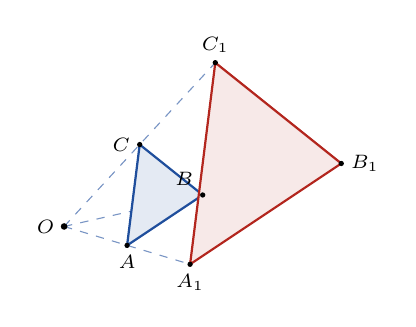
\begin{tikzpicture}[scale=0.8,font=\scriptsize]
\coordinate (O) at (0,0); \coordinate (A) at (1,-0.3); \coordinate (B) at (2.2,0.5); \coordinate (C) at (1.2,1.3);
\coordinate (A1) at (2,-0.6); \coordinate (B1) at (4.4,1); \coordinate (C1) at (2.4,2.6);
\draw[cDef!60,dashed] (O)--(A1) (O)--(B1) (O)--(C1);
\draw[thick,cDef,fill=cDef!12] (A)--(B)--(C)--cycle; \draw[thick,cThm,fill=cThm!10] (A1)--(B1)--(C1)--cycle;
\fill (O) circle (1.5pt) node[left]{$O$};
\foreach \p/\q in {A/below,B/below,C/left,A1/below,B1/right,C1/above} \fill (\p) circle (1.2pt);
\node[below] at (A){$A$}; \node[above left] at (B){$B$}; \node[left] at (C){$C$};
\node[below] at (A1){$A_1$}; \node[right] at (B1){$B_1$}; \node[above] at (C1){$C_1$};
\end{tikzpicture}\end{LTR}\par }{50 د}{الإنشاء بالمسطرة ثم بـ GeoGebra.}
\Row{}{%
\Lab{cThm}{خاصية}\ إذا كانت $M_1$ و $N_1$ صورتي $M$ و $N$:\par\ck\ $\overrightarrow{M_1N_1}=k\overrightarrow{MN}$ و $M_1N_1=|k|\,MN$.\par
\ck\ التحاكي يحافظ على الاستقامية والتوازي والزوايا ، ويحول مستقيماً إلى مستقيم يوازيه.\par
\ck\ صورة دائرة $(O^{\prime};r)$ دائرة مركزها صورة $O^{\prime}$ ونصف قطرها $|k|r$ ؛ المساحات تضرب في $k^2$.\par
\Lab{cRem}{ملاحظات}\ $k=-1$: التناظر المركزي ؛ $k=1$: التحويل المطابق.\par}{}{}
\Row{}{%
\Lab{cThm!80!black}{حذار}\ التحاكي لا يحافظ على المسافات إلا إذا كان $|k|=1$.}{}{}
\Row{التقويم}{%
\Lab{cEx}{تطبيق}\par أنشئ صورة المثلث $ABC$ بالتحاكي $h$ الذي مركزه $A$ ونسبته $-\frac12$. ما نسبة مساحتي المثلثين؟\par\textbf{الحل:} $A_1=A$ ، $\overrightarrow{AB_1}=-\frac12\overrightarrow{AB}$ ، $\overrightarrow{AC_1}=-\frac12\overrightarrow{AC}$ ؛ نسبة المساحتين $\left(-\frac12\right)^2=\frac14$.\par\textbf{واجب منزلي:} تمارين 21 ، 22 ، 23 ، 24 ، 31 من باب التحويلات.\par\smallskip\textbf{ملاحظات حول سير الحصة:} \dotfill}{25 د}{تقويم فردي.}
\end{Sayr}
\newpage
\ModhHead{45}{2 ع ت}{هندسة}{التحويلات النقطية: التحاكي}{02 سا}{استعمال خواص التحاكي: الاستقامية والتوازي}%
{\begin{itemize}\item التحاكي وخواصه.\end{itemize}}%
{\begin{itemize}\item استعمال التحاكي لإثبات استقامية نقط وتوازي مستقيمات.\end{itemize}}%
{المنهاج ، الكتاب المدرسي ، مراجع ، أدوات الهندسة ، برنامج GeoGebra.}
\begin{Sayr}
\Row{مرحلة الانطلاق}{%
\textbf{التهيئة النفسية:} كيف نثبت أن ثلاث نقط على استقامة واحدة؟ (أشعة ، مرجح ، $\ldots$)}{10 د}{تذكير بالطرق.}
\Row{التشخيص والاكتشاف}{%
\Lab{cEx}{مناقشة نشاط 03 صفحة 313}\par\ck\ مثلث $ABC$ ومستقيمات موازية لأضلاعه: نعبّر عن نقطة كمرجح ، ثم نقارن مساحتي مثلثين متحاكيين.\par
}{35 د}{نشاط الكتاب.}
\Row{بناء المعارف}{%
\Lab{cThm}{استقامية}\ النقطة $O$ وأي نقطة $M$ وصورتها $M_1$ بتحاكٍ مركزه $O$ على استقامة واحدة.\par\Lab{cEx}{مركز الثقل}\ $ABC$ مثلث مركز ثقله $G$ ، و $A_1$ ، $B_1$ ، $C_1$ منتصفات $[BC]$ ، $[CA]$ ، $[AB]$.\par\ck\ $\overrightarrow{GA_1}=-\frac12\overrightarrow{GA}$: التحاكي $h(G;-\frac12)$ يحول $A$ إلى $A_1$ ، $B$ إلى $B_1$ ، $C$ إلى $C_1$.\par
\ck\ إذن $(A_1B_1)\parallel(AB)$ و $A_1B_1=\frac12AB$.\par
}{50 د}{نلون المثلثين المتحاكيين.}
\Row{}{%
\Lab{cMeth}{تعيين مركز تحاكٍ}\ إذا كانت $[AB]$ و $[CD]$ متوازيتين وغير متقايستين ، فمركز التحاكي الذي يحول $A$ إلى $C$ و $B$ إلى $D$ هو نقطة تقاطع $(AC)$ و $(BD)$.\par\Lab{cThm!80!black}{حذار}\ نتحقق من النسبة بإشارتها (نفس الاتجاه $k>0$).}{}{}
\Row{التقويم}{%
\Lab{cEx}{تطبيق}\par $ABCD$ شبه منحرف قاعدتاه $[AB]$ و $[CD]$ مع $\overrightarrow{DC}=\frac13\overrightarrow{AB}$ ، والمستقيمان $(AD)$ و $(BC)$ يتقاطعان في $E$. عيّن تحاكياً يحول $A$ إلى $D$ و $B$ إلى $C$.\par\textbf{الحل:} مركزه $E$ ونسبته $\frac13$ لأن $\overrightarrow{DC}=\frac13\overrightarrow{AB}$.\par\textbf{واجب منزلي:} تمارين 38 ، 39 ، 40 ، 42 ، 43 ، 44 ، 46 ، 47 من باب التحويلات.\par\smallskip\textbf{ملاحظات حول سير الحصة:} \dotfill}{25 د}{تقويم فردي.}
\end{Sayr}
\newpage
\ModhHead{46}{2 ع ت}{هندسة}{التحويلات النقطية: التحاكي}{02 سا}{تعيين محل هندسي باستعمال التحاكي}%
{\begin{itemize}\item التحاكي وخواصه ، الدائرة.\end{itemize}}%
{\begin{itemize}\item تعيين مجموعة نقط (محل هندسي) باستعمال التحاكي.\end{itemize}}%
{المنهاج ، الكتاب المدرسي ، مراجع ، أدوات الهندسة ، برنامج GeoGebra.}
\begin{Sayr}
\Row{مرحلة الانطلاق}{%
\textbf{التهيئة النفسية:} نقطة $M$ تتحرك على دائرة: كيف تتحرك منتصف القطعة $[AM]$ حيث $A$ ثابتة؟}{10 د}{محاكاة بـ GeoGebra.}
\Row{التشخيص والاكتشاف}{%
\Lab{cEx}{مناقشة نشاط 04 صفحة 313}\par\ck\ $M$ تمسح دائرة $(C)$ ، والنقطة $N$ مرتبطة بـ $M$ بعلاقة $\overrightarrow{IN}=k\overrightarrow{IM}$.\par
\ck\ نستنتج أن $N$ تمسح دائرة صورة $(C)$ بالتحاكي.\par
}{35 د}{نشاط الكتاب.}
\Row{بناء المعارف}{%
\Lab{cMeth}{طريقة}\ نكتب علاقة شعاعية $\overrightarrow{IN}=k\overrightarrow{IM}$ مع $I$ ثابتة ، فتكون $N$ صورة $M$ بالتحاكي $h(I;k)$ ؛ ومحل $N$ صورة محل $M$.\par\Lab{cEx}{مثال}\ $(C)$ دائرة مركزها $O$ ونصف قطرها $r$ ، $I$ نقطة ثابتة ، و $N$ منتصف $[IM]$ حيث $M\in(C)$.\par\ck\ $\overrightarrow{IN}=\frac12\overrightarrow{IM}$: $N=h(I;\tfrac12)(M)$.\par
\ck\ محل $N$: دائرة مركزها منتصف $[IO]$ ونصف قطرها $\dfrac r2$.\par
}{50 د}{نرسم الدائرتين بلونين.}
\Row{}{%
\Lab{cThm!80!black}{حذار}\ إذا استُثنيت نقط من محل $M$ نستثني صورها من محل $N$.}{}{}
\Row{التقويم}{%
\Lab{cEx}{تطبيق}\par $[AB]$ قطعة ثابتة و $M$ تمسح دائرة مركزها $B$ ونصف قطرها $3$. $G$ مركز ثقل المثلث $ABM$. عيّن محل $G$.\par\textbf{الحل:} $I$ منتصف $[AB]$: $\overrightarrow{IG}=\frac13\overrightarrow{IM}$ ، فـ $G=h(I;\tfrac13)(M)$ ؛ محل $G$ دائرة مركزها صورة $B$ ونصف قطرها $1$ (ماعدا النقطتين المرفقتين بنقطتي تقاطع الدائرة مع $(AB)$).\par\textbf{واجب منزلي:} تمرينا 53 و 54 ، وأعمال موجهة من باب التحويلات.\par\smallskip\textbf{ملاحظات حول سير الحصة:} \dotfill}{25 د}{تقويم فردي.}
\end{Sayr}
\newpage
\ModhHead{47}{2 ع ت}{هندسة}{التحويلات النقطية: التحاكي}{02 سا}{إنشاءات هندسية باستعمال التحاكي}%
{\begin{itemize}\item التحاكي وخواصه.\end{itemize}}%
{\begin{itemize}\item إنجاز إنشاءات هندسية باستعمال التحاكي.\end{itemize}}%
{المنهاج ، الكتاب المدرسي ، مراجع ، أدوات الهندسة ، برنامج GeoGebra.}
\begin{Sayr}
\Row{مرحلة الانطلاق}{%
\textbf{التهيئة النفسية:} كيف نرسم مربعاً داخل مثلث بحيث تكون رؤوسه الأربعة على أضلاعه؟}{10 د}{تحدٍّ إنشائي.}
\Row{التشخيص والاكتشاف}{%
\Lab{cEx}{وضعية مقترحة}\ $ABC$ مثلث. نريد مربعاً $MNPQ$ حيث $M$ و $N$ على $[BC]$ ، $P\in[AC]$ ، $Q\in[AB]$.\par\ck\ نرسم أولاً مربعاً «مساعداً» $M_0N_0P_0Q_0$ له ضلع على $[BC]$ ورأس $Q_0$ على $[AB]$ (دون شرط على $P_0$).\par
}{35 د}{عمل بالأفواج.}
\Row{بناء المعارف}{%
\Lab{cMeth}{الإنشاء}\par\ck\ التحاكي الذي مركزه $B$ يحول المربع المساعد إلى مربع ، ويحافظ على $[BC]$ و $[BA]$.\par
\ck\ المستقيم $(BP_0)$ يقطع $[AC]$ في $P$: هو رأس المربع المطلوب.\par
\ck\ نكمل: $Q$ على $[AB]$ بحيث $(PQ)\parallel(BC)$ ، ثم المسقطان العموديان $M$ و $N$.\par
\Lab{cRem}{ملاحظات}\ فكرة الطريقة: ننشئ شكلاً يحقق كل الشروط إلا شرطاً واحداً ، ثم نستعمل تحاكياً.\par}{50 د}{الإنشاء خطوة خطوة.}
\Row{}{%
\Lab{cThm!80!black}{حذار}\ نبرر أن الشكل الناتج مربع بخواص التحاكي (يحافظ على التوازي والزوايا والنسب).}{}{}
\Row{التقويم}{%
\Lab{cEx}{تطبيق}\par $(C)$ دائرة و $(\Delta)$ مستقيم يقطعها. أنشئ مربعاً له ضلع على $(\Delta)$ ورأسان على $(C)$ ، واشرح الطريقة.\par\textbf{الحل المنتظر:} $H$ المسقط العمودي لمركز الدائرة على $(\Delta)$ ؛ مربع مساعد ضلعه على $(\Delta)$ ومنتصف هذا الضلع $H$ ، ثم التحاكي الذي مركزه $H$ ويرسل رأسه العلوي إلى الدائرة (المستقيم من $H$ نحو الرأس يقطع الدائرة).\par\textbf{واجب منزلي:} تمارين 50 ، 51 ، 52 من باب التحويلات.\par\smallskip\textbf{ملاحظات حول سير الحصة:} \dotfill}{25 د}{نهاية المحور: فرض أو مراجعة.}
\end{Sayr}
\end{document}
